\documentclass[12pt, a4paper]{article}

\usepackage[top=5em, bottom=5em, left=5em, right=5em]{geometry}
\usepackage{enumerate}
\usepackage{graphicx}
\usepackage{listings}
\lstset{
	breaklines=true
}

\setlength\parskip{1em}
\setlength\parindent{0em}

\title{Assignment 2}

\author{Hendrik Werner s4549775}

\begin{document}
\maketitle

\section{} %1
\begin{enumerate}[a]
	\item %a
	I ran "dig @b.root-servers.net cs.ru.nl" and got

	\begin{lstlisting}
; <<>> DiG 9.10.3-P4-Ubuntu <<>> @b.root-servers.net cs.ru.nl
; (2 servers found)
;; global options: +cmd
;; Got answer:
;; ->>HEADER<<- opcode: QUERY, status: NOERROR, id: 56662
;; flags: qr rd; QUERY: 1, ANSWER: 0, AUTHORITY: 8, ADDITIONAL: 17
;; WARNING: recursion requested but not available

;; OPT PSEUDOSECTION:
; EDNS: version: 0, flags:; udp: 4096
;; QUESTION SECTION:
;cs.ru.nl.			IN	A

;; AUTHORITY SECTION:
nl.			172800	IN	NS	ns1.dns.nl.
nl.			172800	IN	NS	ns4.dns.nl.
nl.			172800	IN	NS	ns2.dns.nl.
nl.			172800	IN	NS	ns-nl.nic.fr.
nl.			172800	IN	NS	ns5.dns.nl.
nl.			172800	IN	NS	sns-pb.isc.org.
nl.			172800	IN	NS	nl1.dnsnode.net.
nl.			172800	IN	NS	ns3.dns.nl.

;; ADDITIONAL SECTION:
nl1.dnsnode.net.	172800	IN	A	194.146.106.42
ns1.dns.nl.		172800	IN	A	193.176.144.5
ns2.dns.nl.		172800	IN	A	213.154.241.85
ns3.dns.nl.		172800	IN	A	194.171.17.10
ns4.dns.nl.		172800	IN	A	95.142.99.212
ns5.dns.nl.		172800	IN	A	194.0.28.53
ns-nl.nic.fr.		172800	IN	A	192.93.0.4
sns-pb.isc.org.		172800	IN	A	192.5.4.1
nl1.dnsnode.net.	172800	IN	AAAA	2001:67c:1010:10::53
ns1.dns.nl.		172800	IN	AAAA	2a00:d78:0:102:193:176:144:5
ns2.dns.nl.		172800	IN	AAAA	2001:7b8:606::85
ns3.dns.nl.		172800	IN	AAAA	2001:610:0:800d::10
ns4.dns.nl.		172800	IN	AAAA	2a00:1188:5::212
ns5.dns.nl.		172800	IN	AAAA	2001:678:2c:0:194:0:28:53
ns-nl.nic.fr.		172800	IN	AAAA	2001:660:3005:1::1:2
sns-pb.isc.org.		172800	IN	AAAA	2001:500:2e::1

;; Query time: 170 msec
;; SERVER: 192.228.79.201#53(192.228.79.201)
;; WHEN: Wed Feb 22 14:16:05 CET 2017
;; MSG SIZE  rcvd: 566
	\end{lstlisting}

	Then I ran "dig @ns1.dns.nl cs.ru.nl" and got

	\begin{lstlisting}
; <<>> DiG 9.10.3-P4-Ubuntu <<>> @ns1.dns.nl cs.ru.nl
; (2 servers found)
;; global options: +cmd
;; Got answer:
;; ->>HEADER<<- opcode: QUERY, status: NOERROR, id: 28278
;; flags: qr rd; QUERY: 1, ANSWER: 0, AUTHORITY: 3, ADDITIONAL: 5
;; WARNING: recursion requested but not available

;; OPT PSEUDOSECTION:
; EDNS: version: 0, flags:; udp: 4096
;; QUESTION SECTION:
;cs.ru.nl.			IN	A

;; AUTHORITY SECTION:
ru.nl.			3600	IN	NS	ns1.surfnet.nl.
ru.nl.			3600	IN	NS	ns4.ru.nl.
ru.nl.			3600	IN	NS	ns3.ru.nl.

;; ADDITIONAL SECTION:
ns1.surfnet.nl.		3600	IN	A	192.87.106.101
ns3.ru.nl.		3600	IN	A	131.174.78.16
ns4.ru.nl.		3600	IN	A	131.174.78.17
ns1.surfnet.nl.		3600	IN	AAAA	2001:610:1:800a:192:87:106:101

;; Query time: 9 msec
;; SERVER: 193.176.144.5#53(193.176.144.5)
;; WHEN: Wed Feb 22 14:20:35 CET 2017
;; MSG SIZE  rcvd: 175
	\end{lstlisting}

	which lead me to the final round "dig @ns1.surfnet.nl cs.ru.nl" that produced this

	\begin{lstlisting}
; <<>> DiG 9.10.3-P4-Ubuntu <<>> @ns1.surfnet.nl cs.ru.nl
; (2 servers found)
;; global options: +cmd
;; Got answer:
;; ->>HEADER<<- opcode: QUERY, status: NOERROR, id: 32166
;; flags: qr rd; QUERY: 1, ANSWER: 0, AUTHORITY: 2, ADDITIONAL: 3
;; WARNING: recursion requested but not available

;; OPT PSEUDOSECTION:
; EDNS: version: 0, flags:; udp: 4096
;; QUESTION SECTION:
;cs.ru.nl.			IN	A

;; AUTHORITY SECTION:
cs.ru.nl.		86400	IN	NS	ns1.science.ru.nl.
cs.ru.nl.		86400	IN	NS	ns2.science.ru.nl.

;; ADDITIONAL SECTION:
ns2.science.ru.nl.	86400	IN	A	131.174.16.133
ns1.science.ru.nl.	86400	IN	A	131.174.224.4

;; Query time: 33 msec
;; SERVER: 192.87.106.101#53(192.87.106.101)
;; WHEN: Wed Feb 22 14:21:36 CET 2017
;; MSG SIZE  rcvd: 113
	\end{lstlisting}
	\label{sec:1a}

	\item %b
	Apart from some crazy lines in the output which neither I nor the student assistant could explain the "+trace" option basically does the same as we manually did in (\ref{sec:1a}). It begins at the root servers and traverses down the hierarchy to eventually find the server we requested.

	Most lines looked like this
	\begin{lstlisting}
nl.			172800	IN	NS	nl1.dnsnode.net.
	\end{lstlisting}
	which makes sense but some of them looked like
	\begin{lstlisting}
nl.			86400	IN	RRSIG	DS 8 1 86400 20170307050000 20170222040000 61045 . D4665w6HgEmCnNP/EZdmjQ9bJrMOwqnAQ0gSzVuttj/0bza1SYDuSVUj Nj+ngjkFNf6LKGR40wDZBtDF1m1GHnwaJL1aNcL/twxFqGhOhQLXbroc D0toEvuqwk6r/lYuwDrSm+oXj+dFaRaHRR10csJWYajUWobqsRG6vO0b jLyTeroJuHhiewYjOaVxnkZz38LvdiFTQ8ieEWKtfoJTIVaiAcxviEjp +n/gACvXh2Vxp6BOSIPXMXxt2CKC+i8y1REfF3NekkInI4/cu+k62P3P 8NE1VpwYaP80+dB/pUD4WmqatFurytGfaXz3wiFt2SFLdK5IHbNkm3x8 NcFi1A==
	\end{lstlisting}
	which I do not understand.

	I compared my output to that of a friend and I got all lines he got plus this garbage lines. So at least I am not missing anything.

	After further investigation we found out that there crazy lines contain cryptographic signatures.
\end{enumerate}

\section{} %2
The red section contains the query which asks for cs.ru.nl. The blue section contains the answer.

RFC 1035 specifies an encryption scheme where there can be back references to earlier parts of the message. These back references span 2 bytes and start with "11" followed by a 14 bit offset from the beginning of the message starting at 0.

Excerpt from the RFC:
"In order to reduce the size of messages, the domain system utilizes a
compression scheme which eliminates the repetition of domain names in a
message.  In this scheme, an entire domain name or a list of labels at
the end of a domain name is replaced with a pointer to a prior occurance
of the same name."

The request just asks for "cs.ru.nl". The answer contains the following domains in order:
\begin{itemize}
	\item cs.ru.nl
	\item back reference to cs.ru.nl = cs.ru.nl
	\item mx1.science + backreference to .ru.nl = mx1.science.ru.nl
	\item mx2. + backreference to .science + backreference to .ru.nl = mx2.science.ru.nl
	\item mx3. + backreference to .science + backreference to .ru.nl = mx3.science.ru.nl
	\item ns1. + backreference to .science + backreference to .ru.nl = ns1.science.ru.nl
	\item ns2. + backreference to .science + backreference to .ru.nl = ns2.science.ru.nl
	\item ns3. + backreference to .science + backreference to .ru.nl = ns3.science.ru.nl
\end{itemize}

\section{} %3
\begin{enumerate}[a]
	\item %a
	Host names that need to be resolved
	\begin{enumerate}
		\item .nl
		\item cs.nl
		\item random.cs.nl
		\item www.random.cs.nl
	\end{enumerate}

	\item %b
	The more general the host name is the most likely it will be in the cache. ".nl" is very likely to be cached. "cs.nl" is less likely to be in cache and so on.

	This is because to look up "x.nl" you need to look up ".nl", to look up "y.x.nl" you need to look up "x.nl" so the more top level hosts are more likely to be looked up.

	Another factor might be higher TTLs for higher level DNS host entries. The ip of the ".nl" server probably does not change often so the TTL can be higher.

	\item %c
	If some host shows up in the DNS cache you know that it must have been requested at most TTL seconds ago. This does not actually tell you whether the site has been visited but it can be used as a pretty good indicator because you mostly do DNS requests for hosts you plan t access.

	\item %d
	As mentioned in (b) the hosts whose DNS entries have higher TTLs are more likely to be in cache. This is because once they end up in cache they stay there for longer which means they are at any point more likely to be in cache compared to low TTL hosts DNS entries.

	\item %e
	The FQDN of the printer is "printer.random.cs.nl" and its IP is 134.122.131.10.

	\item %f
	Email is handled by the IMAP protocol. The "imap" DNS entry points to the "alpha" entry which has IP 130.122.131.10. This server will handle email sent to the "random domain".

	\item %g
	A CNAME record points to another name, in this case "alpha". It is better to use a CNAME record here because we only need to update one record (the one for "alpha") when the IP of the server changes. The CNAME records will still point to "alpha" and do not need to be changed.
\end{enumerate}

\section{} %4
With the routines provided in the template implementing traceroute was very easy. You just loop through the TTLs (1..MAX\_HOPS which I had to change because in the provided framework it covers 0..MAX\_HOPS - 1), start a timer ($time.time()$ does not necessarily provide precision $<1$ second so I used $time.perf\_counter()$), build a request with the hostname and current TTL, then send it and stop the timer if the request times out or we receive a response.

Then if you get a response you look up the FQDN of the response's IP and display the FQDN, IP, and RTT. If you do not get a response you just print "*". You repeat that 3 times per TTL.

However the provided $send\_packet\_with\_ttl$ function has a bug. If the request times out it references an undeclared variable. This was easy to fix but I thought we could assume that the code we got from you was correct.

The code is provided as "traceroute.py".

\section{} %5

I executed the following steps:

\begin{lstlisting}
vstart A --eth0=a
vstart B --ath0=b
vstart AB --eth0=a --eth1=b
\end{lstlisting}

For VM $A$:
\begin{lstlisting}
ifconfig eth0 10.0.0.1 up
\end{lstlisting}

For VM $B$:
\begin{lstlisting}
ifconfig eth0 10.0.0.2 up
\end{lstlisting}

For VM $AB$:
\begin{lstlisting}
ifconfig eth0 10.0.0.3 up
ifconfig eth1 10.0.0.4 up
\end{lstlisting}

After that I used $vlist$ to get an overview which produced this output:

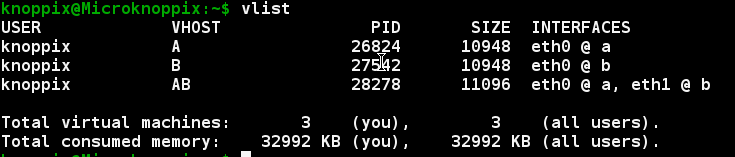
\includegraphics[width=\linewidth]{screenshots/vlist}

The ifconfig output for all VMs is shown here:

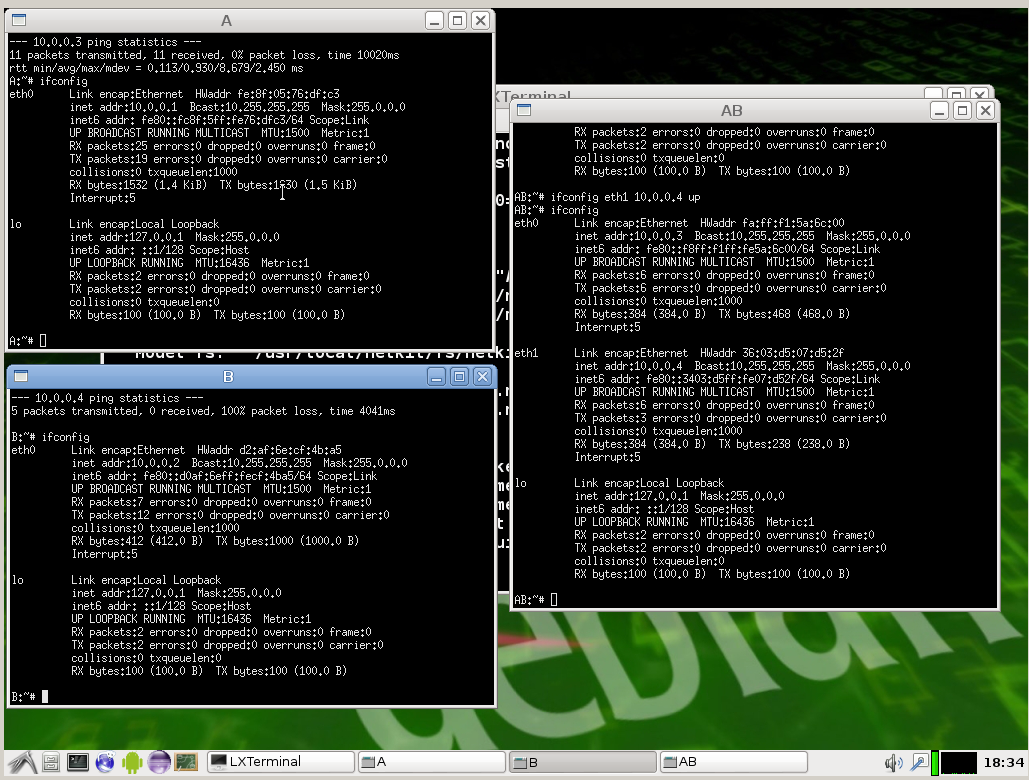
\includegraphics[width=\linewidth]{screenshots/ifconfig}

After this I could ping AB from A and A from AB but B and AB could ping each other. I have no idea at all why this does not work and I even wrote an email to Jon Moroney who wasn't able to help me.

\end{document}
